\documentclass[10pt,xcolor=pdflatex]{beamer}
\usepackage{newcent}
\usepackage[utf8]{inputenc}
\usepackage[czech]{babel}
\usepackage{hyperref}
\usepackage{fancyvrb}
%\usetheme[]{FIT}
\usetheme[CZlogo]{FIT} % CZ logo

%%%%%%%%%%%%%%%%%%%%%%%%%%%%%%%%%%%%%%%%%%%%%%%%%%%%%%%%%%%%%%%%%%
\title[Obhajoba bakalářské práce]{Rozšíření systému pro získávání, zpracování a~analýzu rozsáhlých kolekcí textů z webu}

\author[]{Jiří Matějka}

% \institute[]{Brno University of Technology, Faculty of Information Technology\\
% Bo\v{z}et\v{e}chova 1/2. 612 66 Brno - Kr\'alovo Pole\\
% login@fit.vutbr.cz}

% CZ verzia
\institute[]{Vysoké učení technické v Brně, Fakulta informačních technologií\\
Božetěchova 1/2 612 66 Brno\\
xmatej52@stud.fit.vutbr.cz}


\date{14. 6. 2018}
%\date{\today}
%\date{} % bez data

%%%%%%%%%%%%%%%%%%%%%%%%%%%%%%%%%%%%%%%%%%%%%%%%%%%%%%%%%%%%%%%%%%

\begin{document}

\frame[plain]{\titlepage}

\begin{frame}
  \frametitle{Motivace}
  Dosavadní systém:
  \begin{itemize}
      \item jednorázové vytvoření korpusu z předem shromážděných dat (zatím ověřeno pouze na angličtině)
  \end{itemize}
  Omezení:
  \begin{itemize}
      \item jednotlivé kroky zpracování korpusových dat vyžadují ruční zásahy
      \item nejsou ošetřeny chybové stavy prvotních fází zpracování
      \item není možné korpusová data a indexy snadno aktualizovat
      \item nelze odhadnout, jak dlouho bude zpracování nových dat probíhat
      \item není možné zpracovat dokumenty psané ve více jazycích
      \item v případě chyby se její zdroj hledá velice obtížně
  \end{itemize}
\end{frame}

\begin{frame}
  \frametitle{Zpracování}
  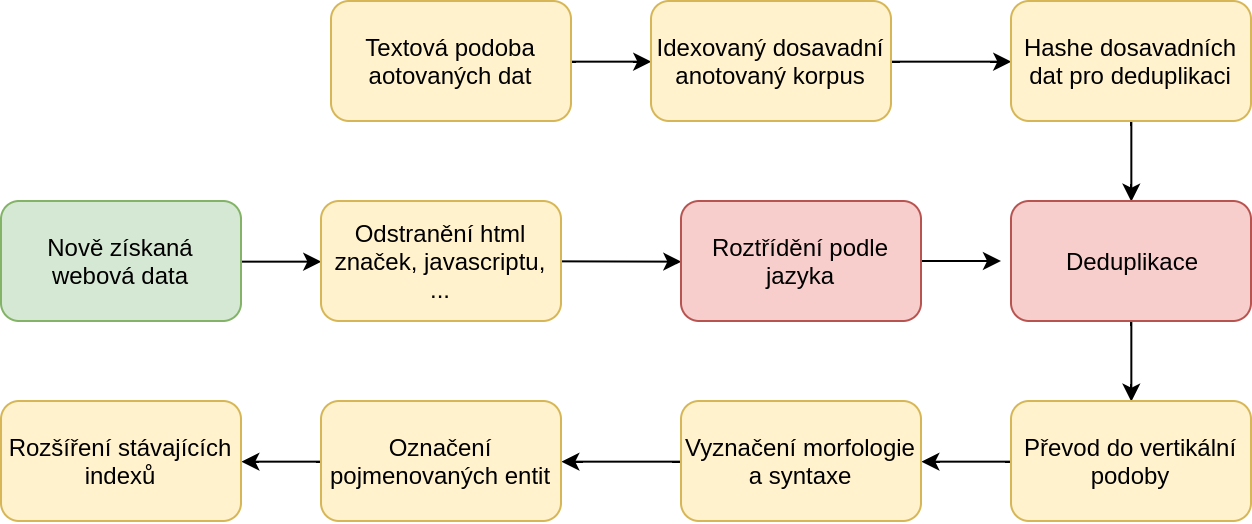
\includegraphics[width=\linewidth]{pipeline.png}
\end{frame}

\begin{frame}
  \frametitle{Rozšíření dosavadního systému}
  Automatizace zpracování:
  \begin{itemize}
      \item vyhledávání nových zdrojů dat
      \item stahování, zpracování a archivace dat
  \end{itemize}
  Logování:
  \begin{itemize}
      \item monitorování běžících procesů zpracování
      \item vedení podrobných a přehledných logů
      \item vedení statistik
      \item pravidelné odesílání emailů o průběhu zpracování
  \end{itemize}
  Zpracování dat:
  \begin{itemize}
      \item zpracování dokumentů psaných ve více jazycích
      \item lepší způsob archivace dat
      \item archiv zpracován více procesy
  \end{itemize}
\end{frame}

\begin{frame}
  \frametitle{Spuštění}
  Spuštění vertikalizace nad již staženými daty (145 GiB):
  \begin{itemize}
      \item 412 minut (nový systém, 12 procesů) $\times$ 354 minut (původní systém, 12 procesů)
      \item bylo ztraceno minimum dat $\times$ data psaná v jiném než českém jazyce byla zahozena
  \end{itemize}
  Spuštění automatického zpracování (3 týdny samostatné činnosti):
  \begin{itemize}
    \item počet RSS a ATOM zdrojů vzrostl ze 116 000 na 185 000
    \item každý den nalezeno v průměru o 15 000 více článků ke stažení
    \item každý den staženo v průměru 10x více článků
    \item během této doby nebyla hlášena žádná chyba (tzn. žádné zpracování neskončilo s chybou)
  \end{itemize}
\end{frame}

\begin{frame}
  \frametitle{Budoucí vývoj}
  Rozšíření automatického zpracování:
  \begin{itemize}
      \item deduplikace vertikalizovaných dat
      \item parsing
      \item tvorba a aktualizce indexů
  \end{itemize}
  Spuštění na více serverech:
  \begin{itemize}
      \item tvorba serveru řídícího zpracování
      \item tvorba klientů provádějící zpracování
  \end{itemize}
\end{frame}

\bluepage{Děkuji za pozornost.}

% Questions
\appendix
\addtocounter{framenumber}{-\value{framenumber}} % Framennumber reset

\begin{frame}
    \frametitle{Otázka oponenta}
    \textbf{Můžete stručně popsat prototyp vytvořeného řešení přiložený na DVD a uvést, proč jste se následně rozhodl dané řešení opustit?}\\[0.5cm]

    Prototyp:
    \begin{itemize}
        \item schopen zpracovat přibližně 70\,\% českých dat.
        \item manuální možnost tvorby indexů
	\end{itemize}
    Nedostatky prototypu:
    \begin{itemize}
        \item schopen zpracovat pouze česká data
        \item manuální obsluha
        \item nástroje mají nepoužitelné a nebo žádné logovací soubory
        \item velká doba zpracování
        \item nevhodný způsob provedení lemmatizace
        \item velká chybovost
	\end{itemize}
\end{frame}

\end{document}
